% \begin{tikzpicture}[node distance=1cm,every node/.style={fill=white, font=\sffamily}, align=center]
%     % Specification of nodes (position, etc.)
%     \node (total)             [large]                                         { };
%     \node (buildable)         [large, below of=total]                         { };
%     \node (testBuildable)     [large, below of=buildable]                     { };
%     \node (success)           [large, below of=testBuildable]                 { };

%     \draw[-Latex]             (total) -- (buildable);
%     \draw[-Latex]             (buildable) -- (testBuildable);
%     \draw[-Latex]             (testBuildable) -- (success);

% \end{tikzpicture}
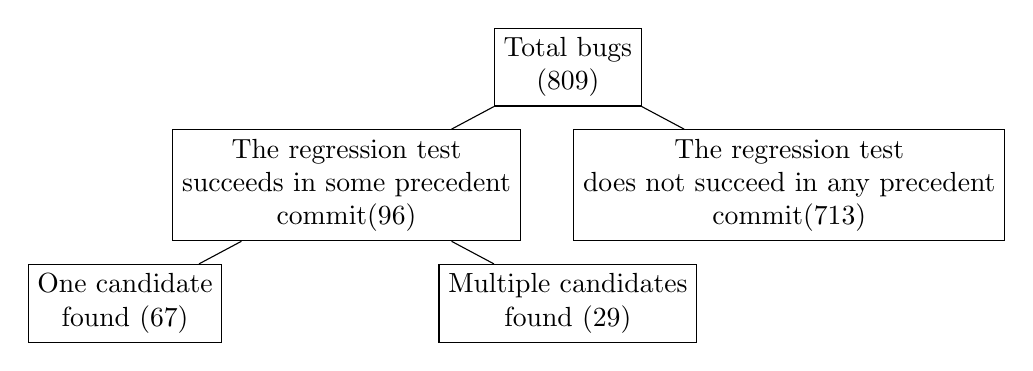
\begin{tikzpicture}[sibling distance=16em,
    every node/.style = {shape=rectangle, draw, align=center, top color=white }]
    \node {Total bugs \\ (809)}
      child { node {The regression test \\ succeeds in some precedent\\ commit(96)} 
          child { node {One candidate\\ found (67)} }
          child { node {Multiple candidates\\ found (29)} }
      }
      child { node {The regression test\\ does not succeed in any precedent\\ commit(713)} }
      ;
\end{tikzpicture}